\section{FDTD}
The Finite Difference Time Domain (FDTD) is a method to numerically solve Maxwell equations in time domain, therefore, it is especially suited for transient analysis and/or for wideband analysis. Generally, it is easy to implement and it scales very good for large simulations, however, it is difficult to simulate curved surfaces with this approach.\\
It is not suited for resonant systems or systems with dispersion. But the material properties ($\mu_r,\epsilon_r$) can be set for every computational node separately!\\ 
Mostly very small simulation time steps are required.

\subsection{Numerical Solution of PDEs}
The general Taylor series expansion of function $f(x,t)$ can be written in numerical form as 
\begin{equation*}
	{f_i}^{n+1}= {f_i}^n + \underbrace{\left(t^{n+1} - t^n\right)}_{\Delta t} \frac{\partial f}{\partial t} \bigg\rvert_{i}^{n} + \frac{1}{2} + \underbrace{\left(t^{n+1} - t^n\right)}_{\left(\Delta t\right)^2} \frac{\partial^2f}{\partial t^2} \bigg\rvert_{i}^{n} \Rightarrow \frac{\partial f}{\partial t} \bigg\rvert_{i}^{n} = \frac{{f_i}^{n+1}-{f_i}^n}{\Delta t} - \underbrace{\frac{1}{2}\Delta t \frac{\partial ^2 f}{\partial t^2}\bigg\rvert_{i}^{n}}_{O(\Delta t)} - \dots
\end{equation*}
This approximation is called first order accurate forward difference approximation. \newline Using a sample in the past and a sample in the future it is possible to increase the precision of the approximation but increase the needed memory (residual error scales down with $\Delta t^2$)
\begin{equation*}
	\frac{\partial f}{\partial t} \bigg\rvert_{i}^{n} = \frac{{f_i}^{n+1}-{f_i}^{n-1}}{\Delta t} - \underbrace{\frac{1}{6}\left(\Delta t\right)^2 \frac{\partial ^3 f}{\partial t^3}\bigg\rvert_{i}^{n}}_{O\left[(\Delta t)^2\right]} - \dots
\end{equation*}
Following the same concept, one can calculate the derivative at half-time-steps:
\begin{equation*}
	\frac{\partial f}{\partial t} \bigg\rvert_{i}^{n+\frac{1}{2}} = \frac{{f_i}^{n+1}-{f_i}^{n}}{\Delta t} - \underbrace{\frac{1}{24}\left(\Delta t\right)^2 \frac{\partial ^3 f}{\partial t^3}\bigg\rvert_{i}^{n}}_{O\left[(\Delta t)^2\right]} - \dots
\end{equation*}
With the same approach the second order centered approximation for the spatial derivation can be written as
\begin{equation*}
	\frac{\partial f}{\partial x} \bigg\rvert_{i}^{n} = \frac{{f_{i+1}}^{n}-{f_{i-1}}^{n}}{2\Delta x} - \underbrace{\frac{1}{6}\left(\Delta x\right)^2 \frac{\partial ^3 f}{\partial x^3}\bigg\rvert_{i}^{n}}_{O\left[(\Delta x)^2\right]} - \dots
\end{equation*}

\subsection{Interlieved Leapfrog (lossless transmission line in this case)}
\begin{minipage}[rt]{9cm}
	\begin{tabular}{l}
		By discretising the voltage at integer grid points\\ (centered at $n+1/2,i$), whilst the current at half grid \\points (centered at $n,i+1/2$): \\
		\begin{equation*}
			V_{i}^{n+1} = V_{i}^{n} - \left(\frac{\Delta t}{C \Delta x}\right) \left[I_{i+1/2}^{n+1/2} - I_{i-1/2}^{n+1/2}\right]
		\end{equation*} \\
		\begin{equation*}
			I_{i+1/2}^{n+1/2} = I_{i+1/2}^{n-1/2} - \left(\frac{\Delta t}{L \Delta x}\right) \left[V_{i+1}^{n} - V_{i}^{n}\right]
		\end{equation*} \\
		Stability for 1D Leapfrog (CFL): \\
		\begin{equation*}
			\Delta t \leq \frac{\Delta x}{|v_p|} \textrm{ where } v_p = \frac{1}{\sqrt{LC}} = \frac{c_0}{\sqrt{\epsilon_r\mu_r}}
		\end{equation*} \\
		General stability (CFL) for dimension $D$ \\if $\Delta x = \Delta y = \Delta z$: \\
		\begin{equation*}
			\Delta t \leq \frac{\Delta x}{\sqrt{\varepsilon \mu}} \cdot \frac{1}{\sqrt{D}} = \frac{\Delta x}{v_p} \cdot \frac{1}{\sqrt{D}}
		\end{equation*}
	\end{tabular}
\end{minipage}
\begin{minipage}[rt]{10cm}
	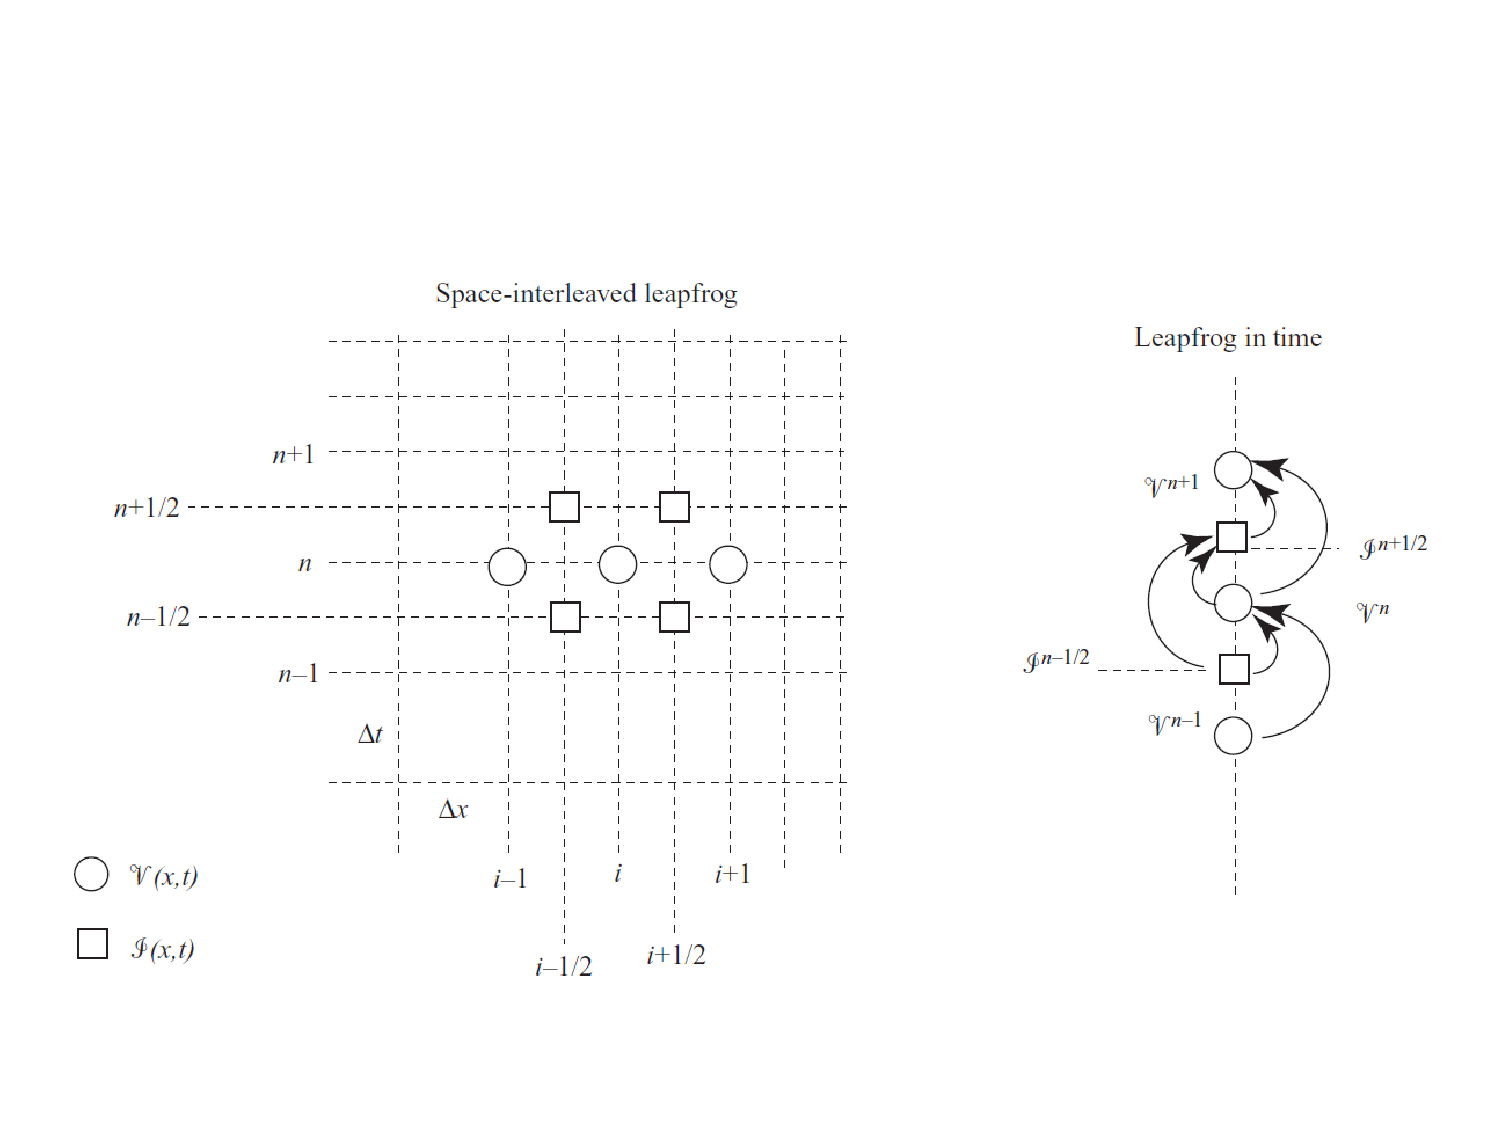
\includegraphics[width=.95\textwidth]{./images/leapfrog.pdf}
\end{minipage}

\subsection{3D Derivation}
\begin{minipage}{12cm}
	The Yee Cell is organized in such a way: \\
	\begin{itemize}
		\item The origin of each cell defines the generic point (i.e. $i,j,k$) at which all vectors are referred to.
		\item The specific component of the electric field is always defined on the \textbf{edges} of the cell containing the origin, displaced by ½ position.
		\item The specific component of the magnetic field is always defined on the \textbf{face} of the cell containing the origin, exactly in the middle.
	\end{itemize}
	Advantages of using the Yee Grid: \\
	\begin{itemize}
		\item Curl equations are automatically satisfied
		\item When considering source free media and second order centered differencing, it can be shown that the Yee cell guaraties divergence difference equations \(\displaystyle \left(\nabla \cdot \vec{B} = 0 \textrm{ (always true)}, \nabla \cdot \vec{E} = 0 \textrm{ (normally true)} \right)\) 
		\item Boundary donditions are automatically satisfied
	\end{itemize}
\end{minipage}
\begin{minipage}{7cm}
	\begin{flushright}
	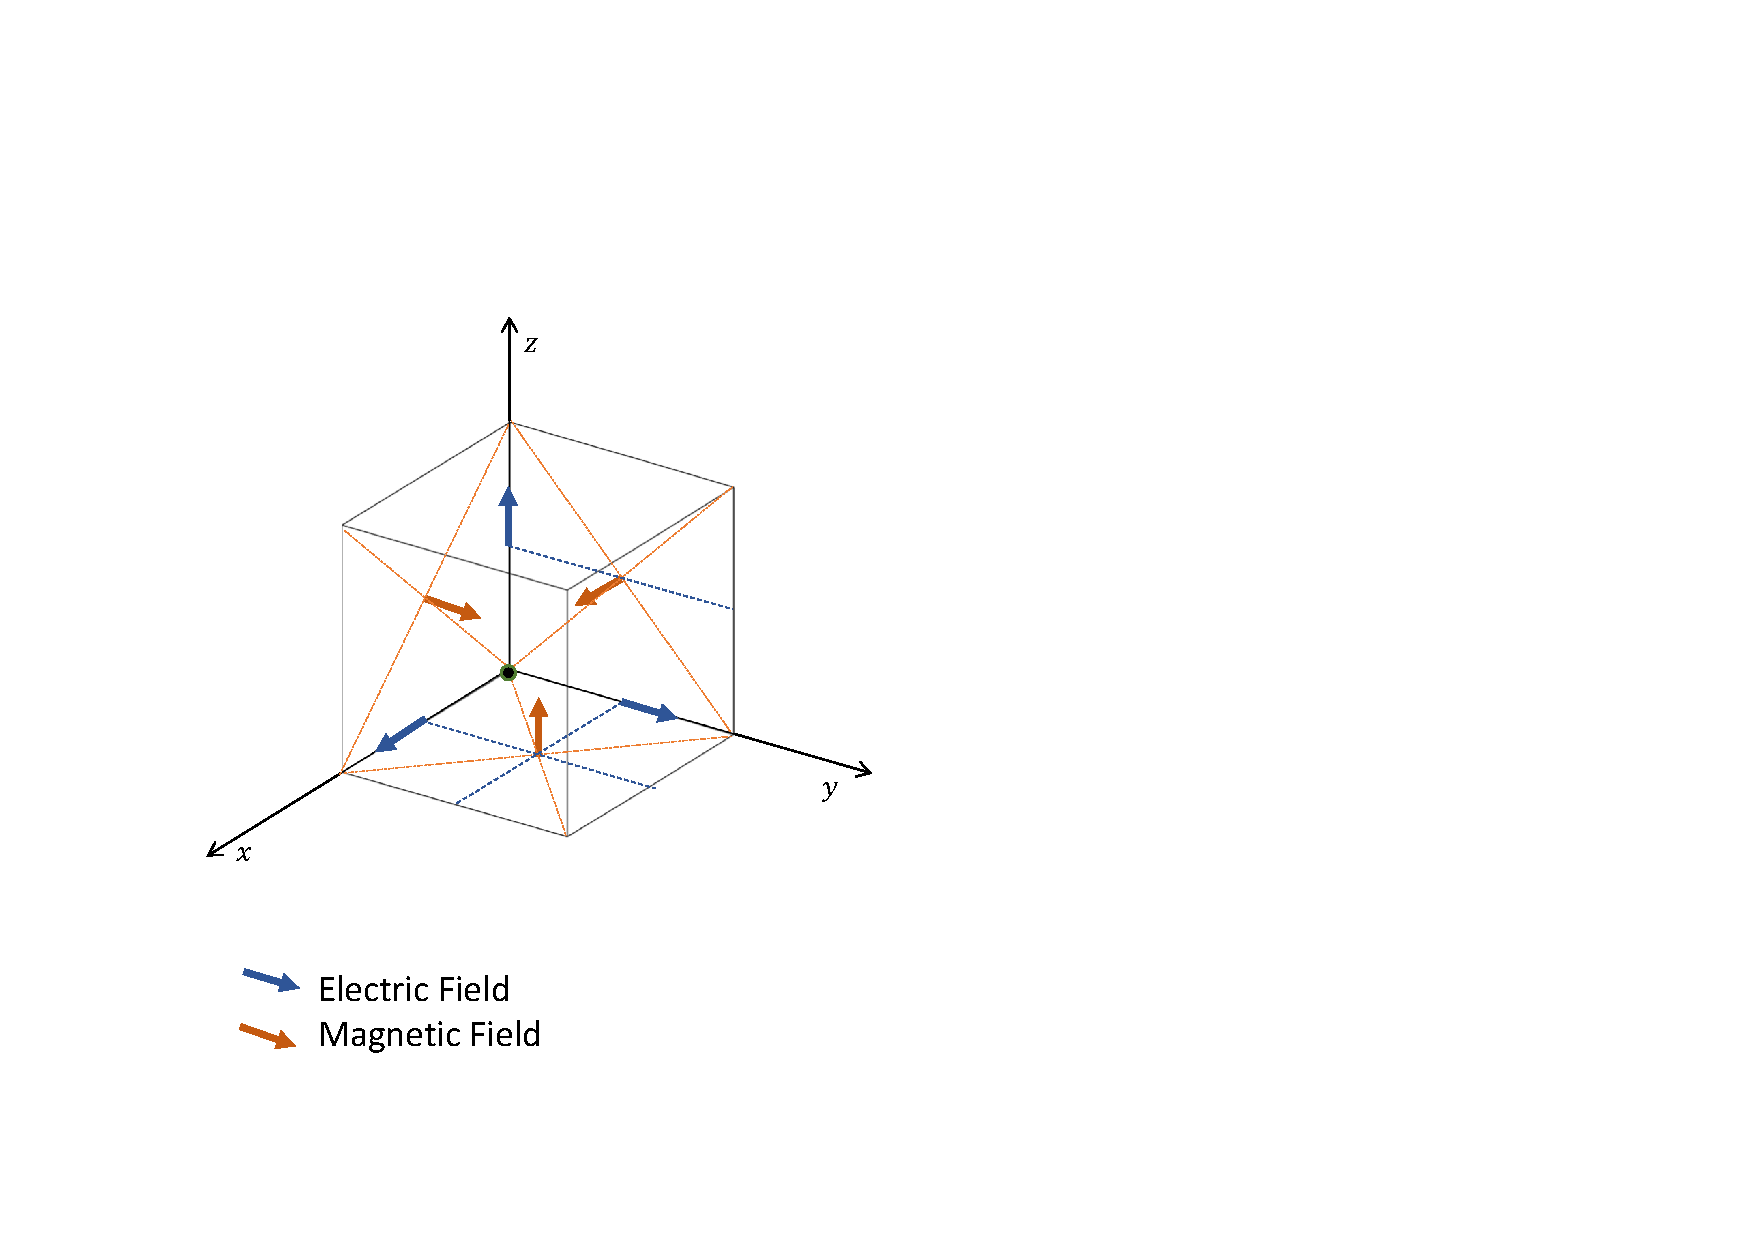
\includegraphics[width=.95\textwidth]{./images/Yee.pdf}
	\end{flushright}
\end{minipage}

\subsection{Normalization of H}
In free space Electric and Magnetic field are related through the characteristic impedance $Z_0$ of free space with
\begin{equation*}
	Z_0 = \frac{E}{H}=\sqrt{\frac{\mu_0}{\varepsilon_0}} \approx 120\pi~\Omega \approx 377~\Omega.
\end{equation*}
This means that the amplitude of the electric field is always at least 377 times bigger than the one of the magnetic field. In order to have a better numeric approximation is common practice to normalize the magnetic field vector using the following expression
\begin{equation*}
	^*\overline{H} = \sqrt{\frac{\mu_0}{\varepsilon_0}} \overline{H}.
\end{equation*}

\subsection{Choice of the time and spatial step}
\label{sec:steps}
The choice of time step is driven by the spatial step and CFL condition. Assuming in general  $\Delta x = \Delta y = \Delta z$ 
\begin{equation*}
	\Delta t \leq \frac{\Delta x}{|v_p|} \cdot \frac{1}{\sqrt{D}}
\end{equation*}
If $\Delta x \neq \Delta y \neq \Delta z$ the following formula should be used:
\begin{equation*}
	\Delta t \leq \frac{1}{|v_p|} \cdot \frac{1}{\sqrt{\Delta x^2+\Delta y^2+\Delta z^2}}
\end{equation*}
the choice of the spatial step is provided by 
\begin{equation*}
	\Delta x \leq \frac{1}{m_\textrm{ovs}} \min (\lambda_\textrm{min},d_\textrm{min})
\end{equation*}
where $m_\textrm{ovs}$ represents the oversampling ratio in spatial domain. Typical values for $m_\textrm{ovs}$ are between 10 and 100. $\lambda_\textrm{min}$ is the smallest wavelength in our system. Generally it is defined as 
\begin{equation*}
	\lambda_\textrm{min} = \frac{v_p}{f_\textrm{max}} = \frac{c_0}{\sqrt{\varepsilon_{r,\textrm{min}}\mu_{r,\textrm{min}}}\cdot f_\textrm{max} }
\end{equation*}
where $v_p$ is the smallest velocity of the wave in any medium of our system, $d_\textrm{min}$ represents the smallest feature dimension we need to simulate and $f_\textrm{max}$ is the maximum frequency of the stimulus.

\subsection{Implementation in MATLAB (1D-FDTD Algorithm)}
How to implement 1D-Maxwell wave equations in MATLAB:\\
\begin{tabular}{l}
	\textbf{1. Initialize E and H vectors to zero}\\
	\includegraphics[width=.6\textwidth]{./images/InitVectors.pdf}\\
	The update coefficients are expressed to calculate *H directly\\
	\textbf{2. Setup time and spatial step}\\
	See chapter \ref{sec:steps}.
	Feature and time steps can only be expressed in integer numbers!! $\rightarrow$ ceil()\\
	\textbf{3. For each time step}\\
	\begin{tabular}{l}
		\hspace{1cm}Setup sources\\
		\hspace{1cm}for each spatial step\\
		\hspace{2cm}update the magnetic field from the electric field\\
		\hspace{2cm} \includegraphics[width=.5\textwidth]{./images/updateH.pdf}\\
		\hspace{2cm}end update H\\
		\hspace{1cm}Setup boundary conditions on H\\
		\hspace{1cm}for each spatial step\\
		\hspace{2cm}update the magnetic field from the electric field\\
		\hspace{2cm} \includegraphics[width=.5\textwidth]{./images/updateE.pdf}\\
		\hspace{2cm}end update H\\
		\hspace{1cm}Setup boundary conditions on H\\
	\end{tabular}
	\\
	\textbf{4.	End loop in time}
\end{tabular}

\subsubsection{Boundary conditions for waves}
\begin{itemize}
	\item \textbf{Total Reflectiong Condition:} The E-Field is set to zero outside the grid. The energy is kept in the grid and bounced back and forth. This assignment is equivalent to the Perfect Electric Conductor (PEC) boundary.\\
	$E(first)=0 \hspace{1cm} E(last) = 0$\\
	Not very useful because there is no PEC existing in nature and the energy remains in the grid what is illogical as well.
	\item \textbf{Periodic Boundary Condition}: Is used for periodic structures. A structures periodicity is reflected in the same periodicity of the E- and H-field.\\
	\begin{minipage}{12cm}
		$E_{first}(Cell 2)=E_{Last}(Cell1)$ \hspace{1cm}and\hspace{1cm} $E_{Last}(Cell 1)=E_{first}(Cell2)$ \\ \\
		And in MATLAB:\\
		\includegraphics[width=0.5\textwidth]{./images/periodic_MATLAB.pdf}\\
		\textbf{Attention!!} $E(1)$ and $E(kStep+1)= E(last)$ are not allowed to be updated
	\end{minipage}
	\begin{minipage}{7cm}
		\begin{flushright}
			\includegraphics[width=1\textwidth]{./images/periodic.pdf}\\
		\end{flushright}
	\end{minipage}
	
	\item \textbf{Absorbing Boundary Condition}: The incident wave will travel through the boundary without reflection. This is specially used at the bounding box. The solution will then be similar as when the bounding box has infinite size $\rightarrow$ smaller bounding boxes can be used.\\
	The Mur boundary is a special absorbing boundary where the wave is artificially cancelled out. Eliminating forward travelling waves: 
	\begin{equation}
	E^{n+1}_1 = E^n_2 - \frac{1-\alpha}{1 + \alpha} \cdot (E^{n+1}_2 + E^n_1 )
	\end{equation}
	Eliminating backward travelling waves:
	\begin{equation}
		E^{n+1}_{last} = E^n_{last-1} - \frac{1-\alpha}{1 + \alpha} \cdot (E^{n+1}_{last-1} + E^n_{last} )
	\end{equation}
	where $\alpha$ is:
	\begin{equation}
		\alpha = \frac{\Delta t}{\Delta z}\cdot c_0
	\end{equation}
	These are the Mur boundary conditions for 1D. \\2D and 3D is much more complicate and Mur boundaries are not suitable. There we use Perfect Matched Layer Boundaries (PMC).
\end{itemize}

\subsubsection{Sources}
A source can be an electric, a magnetic field or a current source. In the last case, the curl equation including the displacement current must be used.
\begin{itemize}
	\item \textbf{Hard Sources}: The source is hardly introduced at specific position in space and the value of the field is substituted (overwritten) with the source value. This is often very useful to modelling antennas because the source appears to the wave like a PEC boundary:\\ \\
	$E_x(SourceZUsed) = src;$
	\\
	\item \textbf{Soft Sources}: The source is superimposed to the field value at a specific position in space. If a wave comes back its value is added to the value of the source. Useful when modelling scattered structures but not ideal because the source sends energy in all directions.\\ \\
	$E_x(SourceZUsed) = E_x(SourceZUsed)+src;$\\
	\item \textbf{TF/SF Source}: This is a kind of soft source called Total Field/Scattered Field source.
	This source has the advantage to travel only in one direction and is transparent for the scattered wave. To implement this, the space is divided in a region where all fields are available (Total Field) and a region where just the scattered field is available.\\This can be achieved by updating the E and H-equations with an additional term:\\ \\
	$E_x(SourceZUsed) = E_x(SourceZUsed)+UC_Ex(SourceZUsed)*src;$\\
	$H_y(SourceZUsed) = H_y(SourceZUsed)+UC_Hy(SourceZUsed)*src;$\\
\end{itemize}

